\documentclass{beamer}
\usepackage[utf8]{inputenc}
\usetheme{Copenhagen}
\usepackage[spanish]{babel}
\usepackage{multirow}
%\usepackage{estilo-apuntes}
\usepackage{braids}
\usepackage[]{graphicx}
\usepackage{pgf,tikz}
\usepackage{pgfplots}
\pgfplotsset{compat=1.13}
\usetikzlibrary{decorations.shapes}
\pgfkeyssetvalue{/tikz/braid height}{1cm} %no parece hacer nada
\pgfkeyssetvalue{/tikz/braid width}{1cm}
\pgfkeyssetvalue{/tikz/braid start}{(0,0)}
\pgfkeyssetvalue{/tikz/braid colour}{black}

\theoremstyle{definition}

\newtheorem{teorema}{Teorema}
\newtheorem{defi}{Definición}
\newtheorem{prop}[teorema]{Proposición}

\newcommand{\C}{\mathbb{C}}
\newcommand{\D}{\mathbb{D}}
\providecommand{\gene}[1]{\langle{#1}\rangle}


\addtobeamertemplate{navigation symbols}{}{%
    \usebeamerfont{footline}%
    \usebeamercolor[fg]{footline}%
    \hspace{1em}%
    \insertframenumber/\inserttotalframenumber
}
\setbeamercolor{footline}{fg=black}
\setbeamerfont{footline}{series=\bfseries}

%-----------------------------------------------------------

\title{El problema de la palabra en los grupos de trenzas}
\author{Javier Aguilar Martín}
\institute{Universidad de Sevilla}
\date{}
 
\begin{document}
\frame{\titlepage}
%\begin{frame}
%
%
%\title[About Beamer] %optional
%{About the Beamer class in presentation making}
% 
%\subtitle{A short story}
% 
%\author[Arthur, Doe] % (optional, for multiple authors)
%{A.~B.~Arthur\inst{1} \and J.~Doe\inst{2}}
% 
%\institute[VFU] % (optional)
%{
%  \inst{1}%
%  Faculty of Physics\\
%  Very Famous University
%  \and
%  \inst{2}%
%  Faculty of Chemistry\\
%  Very Famous University
%}
% 
%\date[VLC 2013] % (optional)
%{Very Large Conference, April 2013}


%\end{frame}

%\AtBeginSection[]{
\begin{frame}
\frametitle{Tabla de contenidos}
\tableofcontents
\end{frame}
%}

\section{El problema de la palabra}

\begin{frame}
\frametitle{El problema de la palabra}
Sea $G=\gene{S\mid R}$. Dados $A,B\in G$ expresados como producto de los generadores de $G$ y sus inversos
\[
\mbox{¿}A=B?\Leftrightarrow \mbox{¿}AB^{-1}=1?
\]
\end{frame}

\section{Definiciones de los grupos de trenzas}

\subsection{Trenzas geométricas}

\begin{frame}
\frametitle{Trenzas geométricas}
\begin{defi}\label{geo}
Denotemos $\Sigma_n$ al grupo simétrico sobre $n$ elementos. Sean $n$ puntos $P_1,\dots, P_n\in\C$ (se puede suponer que $P_k=k$). Se define la \textbf{trenza geométrica} de $n$ cuerdas como la $n$-upla $\beta=(\beta_1,\dots,\beta_n)$ de caminos $\beta_k:[0,1]\to\C\times[0,1]$ tal que:
\begin{itemize}
\item<1-> $\beta_k(0)=(P_k,0)$,
\item<2-> existe una permutación $\tau=\tau(\beta)\in\Sigma_n$ tal que $\beta_k(1)=(P_{\tau(k)},1)$, llamada \textbf{permutación inducida} por $\beta$,
\item<3-> $\beta_k(t)\neq \beta_l(t)$ para todo $k\neq l$ y para todo $t\in[0,1]$.
\item<4-> $\beta_k(t)$ es monótona creciente en la segunda coordenada. 
\end{itemize}
\end{defi}
\end{frame}

\begin{frame}
\begin{figure}[h!]
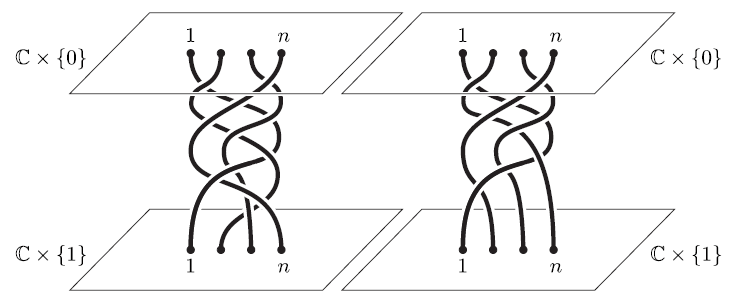
\includegraphics[scale=0.5]{Imagenes/hilos}
\caption{Una trenza geométrica pura y una trenza geométrica no pura.}
\end{figure}
\end{frame}

\begin{frame}
\frametitle{Representación plana}
\begin{figure}[h!]
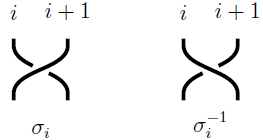
\includegraphics[scale=0.6]{Imagenes/Diapcruce}
\caption{Cruce positivo y cruce negativo.}
\end{figure}
\end{frame}

\begin{frame}
\begin{figure}[h!]
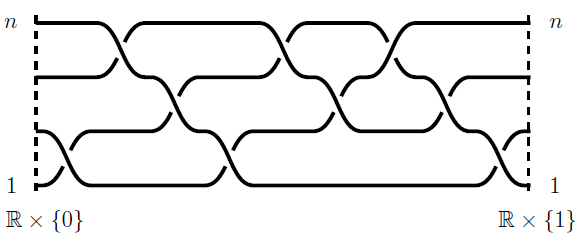
\includegraphics[scale=0.6]{Imagenes/Diapplana}
\caption{Representación plana de una trenza.}
\end{figure}
\end{frame}

\begin{frame}
\frametitle{Concatenación}
\begin{figure}[h!]
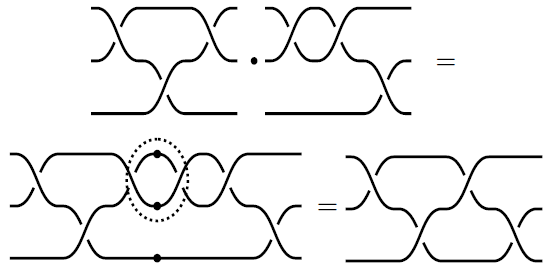
\includegraphics[scale=0.6]{Imagenes/Diapconca}
\caption{Concatenación de trenzas.}
\end{figure}
Esta operación induce un producto entre las clases de homotopía.
\end{frame}

\begin{frame}
Denotemos $B_n$ al conjunto de clases de homotopía relativa a los extremos de trenzas de $n$ cuerdas y $PB_n$ al conjunto de clases de homotopía relativa a los extremos de trenzas puras de $n$ cuerdas.

\begin{prop}
El conjunto $B_n$ dotado de la operación inducida por la concatenación tiene estructura de grupo, al que se le llama \textbf{grupo de trenzas} de $n$ cuerdas. El resultado también es cierto para $PB_n$, cuyo nombre es \textbf{grupo de trenzas puras} de $n$ cuerdas. 
\end{prop}
\end{frame}


\subsection{Espacios de configuración}

\begin{frame}
\frametitle{Espacios de configuración}
\begin{defi}
Dado un espacio topológico $X$, el $n$-ésimo \textbf{espacio de configuración} de $X$ se define como el conjunto
$$M_n(X)=\{(x_1,\dots,x_n)\in X^n\mid x_i\neq x_j\ \forall i\neq j\},$$
dotado de la topología relativa de $X^n$.
\end{defi}
\begin{defi}
Se define el $n$-ésimo \textbf{espacio de configuración no ordenado} de $X$ como el espacio de órbitas
$$N_n(X)=M_n(X)/\Sigma_n.$$
\end{defi}
\end{frame}

\begin{frame}
NO SÉ SI PONER TAMBIÉN AQUÍ LAS REFERENCIAS 
\begin{teorema}
El grupo de trenzas puras de $n$ cuerdas es
$$PB_n=\pi_1(M_n(\C))$$
y el grupo de trenzas de $n$ cuerdas es
$$B_n=\pi_1(N_n(\C)).$$
\end{teorema}
\end{frame}

\subsection{Mapping class groups}

\begin{frame}
\frametitle{Mapping class groups}
\begin{defi}
Una \textbf{isotopía} entre dos espacios topológicos $X$ e $Y$ es una familia continua de homeomorfismos $h_t:X\to Y$ con $0\leq t\leq 1$. Dos homeomorfismos $f,g:X\to Y$ son \textbf{isotópicos} si existe una isotopía $h_t:X\to Y$ con $h_0=f$ y $h_1=g$. 
\end{defi}
Sea $Homeo^+(\D_n)$ el conjunto de homeomorfismos que preservan la orientación de $\D_n$ en sí mismo, fijando los puntos del borde. 
\end{frame}


\begin{frame}
Consideraremos que dos automorfismos son iguales si pueden ser transformados el uno en el otro mediante una isotopía de $\D_n$ en sí mismo que fije el borde y los agujeros.
\begin{defi} Si denotamos $Homeo^+_0(\D_n)$ a la clase de equivalencia de $Id_{\D_n}$ en $Homeo^+(\D_n)$, definimos entonces el \textbf{mapping class group} (grupo de clases de aplicaciones) de $\D_n$ como:
$$\mathcal{M}(\D_n)=Homeo^+(\D_n)/Homeo^+_0(\D_n).$$
\end{defi}
\end{frame}

\subsection{Presentación del grupo de trenzas}



\begin{frame}
\frametitle{Presentación del grupo de trenzas}
\[
B_n=\left\langle\begin{array}{c| c c}
\multirow{2}{*}{$\sigma_1,\dots,\sigma_{n-1}$} & \sigma_i\sigma_j=\sigma_j\sigma_i, & |i-j|>1\\
& \sigma_i\sigma_j\sigma_i=\sigma_j\sigma_i\sigma_j, & |i-j|=1
\end{array}\right\rangle
\]
\end{frame}

\begin{frame}
\frametitle{Presentación del grupo de trenzas puras}
Se definen los generadores 
\[
A_{ij}=\sigma_{j-1}\dots\sigma_{i+1}\sigma_i^2\sigma_{i+1}^{-1}\dots\sigma_{j-1}^{-1}\ (1\leq i<j\leq n)
\]
y las relaciones
\begin{align*}
A_{ij}^{-1}A_{rs}A_{ij}&=A_{rs}\text{ si } (i<j<r<s)\text{ o bien } (r+1<i<j<s),\\
A_{ij}^{-1}A_{js}A_{ij}&=A_{is}A_{js}A_{is}^{-1} \text{ si } (i<j<s),\\
A_{ij}^{-1}A_{is}A_{ij}&=A_{is}A_{js}A_{is}A_{js}^{-1}A_{is}^{-1}\text{ si } (i<j<s),\\
A_{ij}^{-1}A_{rs}A_{ij}&=A_{is}A_{js}A_{is}^{-1}A_{js}^{-1}A_{rs}A_{js}A_{is}A_{js}^{-1}A_{is}^{-1}\text{ si } (i+1<r<j<s).
\end{align*}
\end{frame}

\section{Automorfismos del grupo libre}
\begin{frame}
\frametitle{Automorfismos del grupo libre}
\end{frame}

\begin{frame}
Poner la expresión de la presentación y los dibujitos
\end{frame}

\begin{frame}
\frametitle{Solución al problema de la palabra}
\end{frame}

\section{Peinado de trenzas}
\begin{frame}
\frametitle{Peinado de trenzas}
\end{frame}

\end{document}
